\section{Introduction}

While Lionel Messi's legacy is intrinsically tied to his accomplishments with 
FC Barcelona, his journey with the Argentina national team presents a different 
facet of his illustrious career. This chapter delves into Messi's complex and 
captivating history representing his home country.
From early promise to heartbreaking defeats and ultimately, the pinnacle of 
international success, this exploration provides a comprehensive understanding 
of Messi's impact on Argentine football. 

We begin by tracing Messi's early involvement with the national team, 
highlighting his rise through the youth ranks \parencite[e.g.,][]{messi2005u20wc} 
and his debut with the senior squad.
The narrative then delves into the various tournaments Messi participated in, 
analyzing his performances and the team's overall results. Particular emphasis 
is placed on the Copa América and the FIFA World Cup, where Messi faced immense 
pressure and scrutiny.

Finally, the chapter culminates with an in-depth analysis of Argentina's 
historic victory in the 2022 World Cup, examining the factors that contributed 
to their triumph and Messi's pivotal role in achieving this long-awaited glory.
This chapter aims to provide a balanced perspective on Messi's international 
career, acknowledging both the challenges he faced and the ultimate redemption 
he achieved.

\section{Early Years and Rise in the National Team}

Messi's association with the Argentina national team began at a young age.
He represented Argentina in various youth tournaments, showcasing his 
exceptional talent and quickly establishing himself as a rising star.
His performances at the 2005 FIFA World Youth Championship, where he led 
Argentina to victory and earned the Golden Ball and Golden Shoe awards, 
signaled his immense potential on the international stage. 

Messi's senior debut for Argentina came in 2005, and he quickly became an 
integral part of the team. However, early success in youth tournaments did 
not immediately translate to similar triumphs with the senior squad.
Despite Messi's individual brilliance, Argentina faced several setbacks in 
major tournaments, including Copa América and the World Cup. 

\section{Challenges and Heartbreaks}

Messi's international career was marked by a series of near misses and 
disappointments.
Argentina reached the Copa América final in 2007, 2015, and 2016, only to 
fall short each time.
The 2014 World Cup final defeat to Germany was another agonizing moment for 
Messi and the team. 

\begin{figure}[ht!]
    \centering
    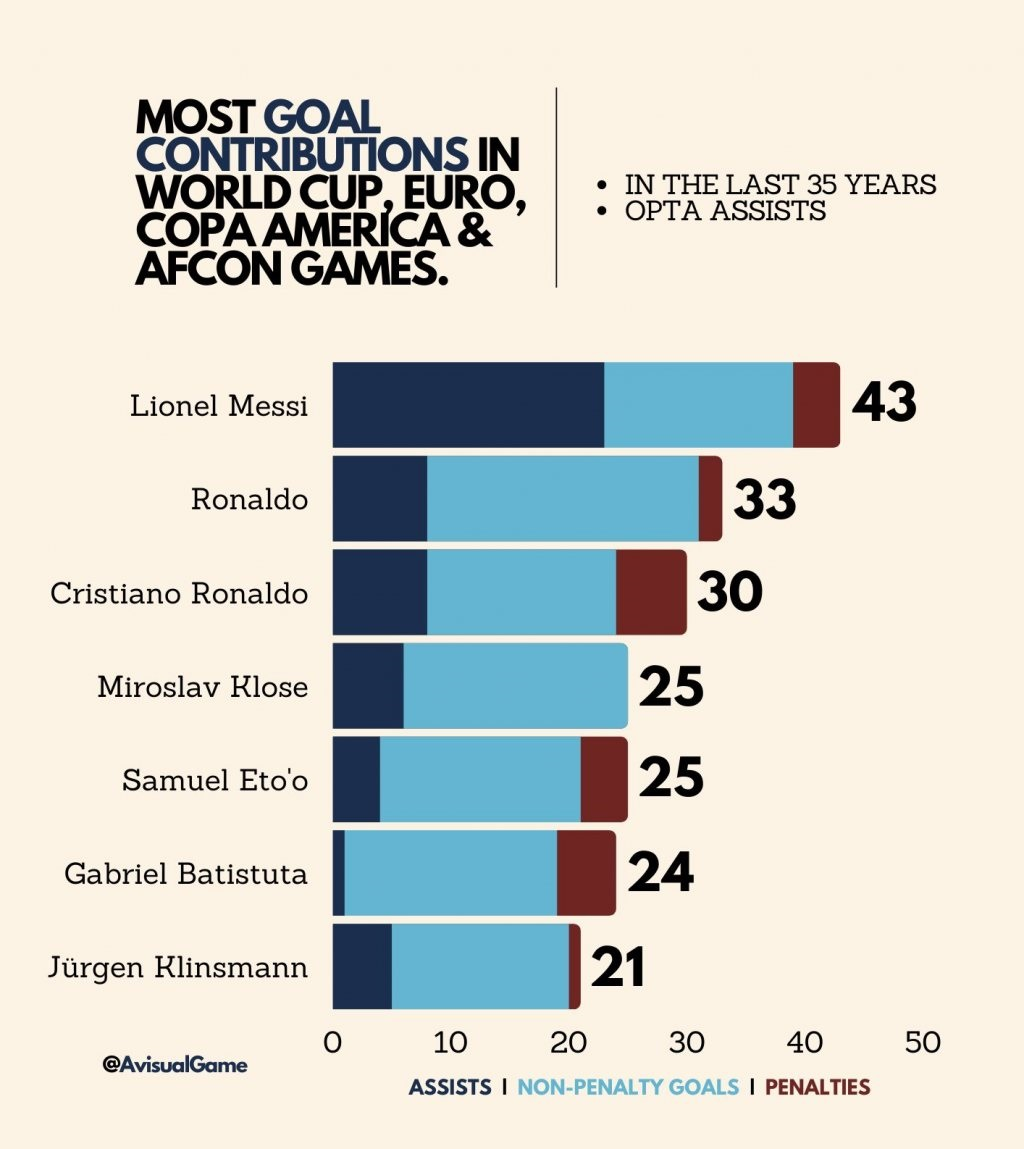
\includegraphics[width=0.6\textwidth]{chapter_two/graphics/international_contributions.jpg}
    \caption{Messi's International Contributions among Top Players}
    \label{fig:international_contributions}
    \begin{quote}
        \textit{Notes:} 
        The figure shows top international contributions in the 
        last 35 years including the World Cup and the main 
        continental tournaments.
        \textit{Source:} Twitter, @avisualgame 
    \end{quote} 
\end{figure}


These defeats led to intense scrutiny and criticism, with some questioning 
Messi's leadership and ability to replicate his club success with the national
team.
The pressure on Messi was immense, as the hopes of a nation rested on his 
shoulders.
All of this despite his consistent performances and contributions, which
can be noticed in Figure \ref{fig:international_contributions}.

\section{The 2022 World Cup Triumph}

Lionel Scaloni's appointment as the national team coach marked a turning point
in Messi's international career.
With him, Messi achieved the Copa América victory in 2021, breaking the
long-standing trophy drought for Argentina, and the Finalissima against 
Italy in 2021 \parencite{messi2021copa, messi2022finalissima}.
However, the ultimate prize remained the FIFA World Cup, a tournament that had
eluded Messi throughout his career, which he finally won in 2022
\parencite{messi2022wc}.
Messi, at the age of 35, led the team with exceptional performances, scoring 
crucial goals and providing assists throughout the tournament.

The final against France \parencite{france2022wc} was a dramatic affair, with 
Argentina emerging victorious after a penalty shootout.
This triumph marked the culmination of Messi's long and arduous journey with 
the national team.
He had finally achieved the ultimate prize in international football, cementing 
his status as one of the greatest players of all time.

\begin{figure}[ht!]
    \centering
    
\includegraphics[width=0.65\textwidth]{chapter_two/graphics/messi_world_cup.jpg}
    \caption{Messi lifting the World Cup trophy}
    \label{fig:international_contributions}
    \begin{quote}
        \textit{Notes:} 
        The picture shows Lionel Messi and his teammates celebrating their victory 
        in the 2022 FIFA World Cup.
    \end{quote} 
\end{figure}


\section{Legacy and Impact}

Lionel Messi's impact on Argentine football extends far beyond trophies and 
accolades.
He has inspired generations of young players and instilled a sense of belief in
the national team. His dedication, resilience, and unwavering passion for 
representing his country have left an indelible mark on the sport.

Messi's journey with Argentina is a testament to the power of perseverance and 
the pursuit of dreams.
Despite facing numerous challenges and setbacks, he never gave up on his 
ambition to bring glory to his nation. His story will continue to inspire 
aspiring footballers and fans worldwide for years to come.
